	\newpage
\section{Projektowanie}		%3
%Opis przygotowania narzędzi (git, visual studio). Wybór i opis bibliotek, klas. Szkic layoutów. Pseudo kody. Opisy wykorzystanych algorytmów (np. algorytm sortowania). Dokładniejsze określenie założeń i działania aplikacji, (np.: ten przycisk otworzy takie okno a w tym oknie wpisujemy takie dane).

\subsection{Wykorzystane narzędzia}

Podczas tworzenia aplikacji, której docelowym środowiskiem będzie Android wykorzystaliśmy platformę open source Xamarin i zestaw narzędzi Xamarin Community Toolkit, który ułatwił wykonywanie niektórych zadań. Projekt jest tworzony~w języku C\# co umożliwia nam wykorzystanie Microsoft Visual Studio Community Edition 2022. IDE (z ang. Integrated Development Environment), czyli zintegrowane środowisko programistyczne posłuży nam do łatwiejszego modułowania aplikacji. Wszystkie wersje kodów aplikacji znajdują się na platformie GitHub dzięki czemu łatwiej będzie wrócić do poprzednich wersji aplikacji w przypadku wystąpienia błędów w działaniu aktualnej. Wszystko początkowo miało zostać połączone za pomocą bazdy danych Firebase. Baza ta umożliwiałaby przesyłanie danych między graczami i ułatwiała przejście do następnych poziomów.

\subsubsection{Xamarin}

Xamarin\footnote{http://xamarinlab.pl/\cite{www1}} (logo - rys. 3.1) to platforma typu open source do tworzenia nowoczesnych i wydajnych aplikacji dla systemów iOS, Android i Windows za pomocą platformy .NET. Xamarin to warstwa abstrakcji, która zarządza komunikacją udostępnionego kodu z bazowym kodem platformy. Środowisko Xamarin działa w środowisku zarządzanym, które zapewnia wygody, takie jak alokacja pamięci i odzyskiwanie pamięci.

	\begin{figure}[!htb]
	\begin{center}
		
\includegraphics[width=8cm]{rys/xamarin.png}
		\caption{Xamarin}
		\label{rys:rysunek001}
	\end{center}
\end{figure}

\subsubsection{Xamarin Community Toolkit}

Zestaw narzędzi Xamarin Community Toolkit\footnote{https://learn.microsoft.com/pl-pl/xamarin/community-toolkit/\cite{www2}} (logo - rys 3.2) to zbiór elementów wielokrotnego użytku na potrzeby tworzenia aplikacji mobilnych za pomocą zestawu narzędzi Xamarin.Forms, w tym animacji, zachowań, konwerterów, efektów i pomocników. Upraszcza i demonstruje typowe zadania deweloperskie podczas kompilowania aplikacji dla systemów iOS, Android, macOS, WPF i platforma uniwersalna systemu Windows (UWP) przy użyciu platformy Xamarin.Forms.

	\begin{figure}[!htb]
	\begin{center}
		
\includegraphics[width=8cm]{rys/xtools.png}
		\caption{Xamarin Community ToolKit}
		\label{rys:rysunek001}
	\end{center}
\end{figure}

\subsubsection{Microsoft Visual Studio}

Microsoft Visual Studio\footnote{ https://visualstudio.microsoft.com/pl\cite{www3}} (logo - rys 3.3) to zintegrowane środowisko programistyczne, służące do tworzenia, edytowania i debugowania kodu. IDE (z ang. Integrated Development Environment), czyli zintegrowane środowisko programistyczne to software oferujący szereg funkcji przydatnych podczas tworzenia oprogramowania dla systemów Windows, Android, iOS, rozwiązań internetowych oraz opartych o~chmurę. Poza standardowym edytorem oraz debugerem, które zapewnia większość aplikacji IDE, program Microsoft Visual Studio zawiera jeszcze kompilatory, narzędzia do uzupełniania kodu i wiele innych funkcji usprawniających pracę.
\\
\\
\\
\\
\\
\\
\\
\\
\\
\\
	\begin{figure}[!htb]
	\begin{center}
		
\includegraphics[width=8cm]{rys/visual.png}
		\caption{Visual}
		\label{rys:rysunek001}
	\end{center}
\end{figure}

\subsubsection{Git, GitHub}

Git jak i GitHub\footnote{ https://github.com/\cite{www4}}  (logo - rys 3.4) to najczęściej używany nowoczesny system kontroli wersji. Za pomocą usługi Git możesz śledzić zmiany kodu wprowadzane w~czasie i przywrócić określone wersje. Ponadto pozwala kontrolować dostęp do danych, wspiera zarządzanie wieloma repozytoriami. Jest to rozwiązanie, które pozwala zaoszczędzić sporo czasu i nerwów. Kolejnym plusem jest to, że jest on w~miare łatwy w użyciu i jest przejrzysty. 
\\
\\
\\
\\
\\
\\
\\
\\
\\
	\begin{figure}[!htb]
	\begin{center}
		
\includegraphics[width=8cm]{rys/git.png}
		\caption{GitHub}
		\label{rys:rysunek001}
	\end{center}
\end{figure}


\subsubsection{Język C\#}

Język C\#\footnote{ https://learn.microsoft.com/pl-pl/dotnet/csharp/\cite{www5}} (logo - rys 3.5) to zorientowany obiektowo język programowania, który umożliwia programostom tworzenie różnych bezpiecznych i niezawodnych aplikacji w środowisku .NET. Język ten udostępnia konstrukcje językowe, które bezpośrednio obsługują te koncepcje, dzięki czemu język C\# jest językiem naturalnym, w którym można tworzyć składniki oprogramowania i ich używać.
\\
\\
\\
\\
\\
\\
\\
\\
\\
\\
\\
\\
\\
\\
\\
\\
\\
\\
	\begin{figure}[!htb]
	\begin{center}
		
\includegraphics[width=8cm]{rys/c.png}
		\caption{C\#}
		\label{rys:rysunek001}
	\end{center}
\end{figure}
\subsubsection{Baza danych SQLite}
SQLite\footnote{ https://www.sqlite.org/index.html/\cite{www6}} (logo - rys 3.6) jest bez serwerową, relacyjną, lekką bazą danych. Znajduje się w dokładnie jednych pliku. Bardzo często wybierana jako baza dla aplikacji iOS oraz Android. 
Zawartość bazy danych przetrzymywana jest w jednym pliku. Baza SQLite jest utrzymywana na dysku przy użyciu B-drzew. Osobne drzewo jest używane dla każdej z tabel i każdego z indeksów. Baza udostępnia transakcje ACID oraz implementuje większość standardu SQL 92. Jest często wykorzystywany w większych aplikacjach oraz w systemach obsługi relacyjnych baz danych takich jak Kexi.
\\
	\begin{figure}[!htb]
	\begin{center}
		
\includegraphics[width=8cm]{rys/baza.png}
		\caption{Komunikat błędu}
		\label{rys:rysunek001}
	\end{center}
\end{figure}
\\
\subsection{Działanie aplikacji}
\textbf{ Gra zawiera kilka paneli: }
\begin{itemize}
	\item \textbf{Menu główne}
	\item \textbf{Menu ustawień} 
	\item   \textbf{Dwa tryby gry}
	\begin{itemize}
		\item \textbf{Tryb graficzny}
		\item \textbf{Tryb tekstowy} 
	\end{itemize}
\end{itemize}


\subsubsection{Menu główne}
Po uruchomieniu aplikacji powita nas już pierwsza zagadka (rys 3.7), która polega na znalezienu przycisku pozwalającego przejść dalej. Tym przyciskiem jest przycisk oznaczony żarówką. Jeśli jednak zostanie wciśnięty duży czerwony przycisk na środku ekranu to gra zostanie wyłączona. 
\\Jak widać mamy dostępny jeszcze przycisk oznaczony zębatką. Prowadzi on do ustawień rozgrywki.
\\
\\
\\
\\
\\
\\
\\
\\
\\
\\
\\
\\
\\
\\
\\
\\
\\
\\
	\begin{figure}[!htb]
	\begin{center}
		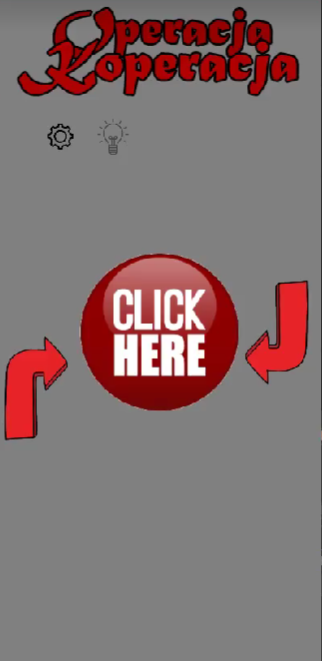
\includegraphics[width=8cm]{rys/menu1.png}
		\caption{Menu Główne}
		\label{rys:rysunek001}
	\end{center}
\end{figure}

	\begin{figure}[!htb]
	\begin{center}
		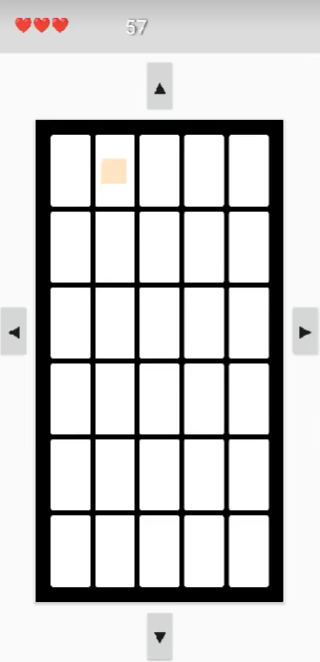
\includegraphics[width=8cm]{rys/menu12.png}
		\caption{Menu Główne v2}
		\label{rys:rysunek001}
	\end{center}
\end{figure}

\hspace{-0.60cm}Po wciśnięciu dobrego przycisku przechodzimy do właściwego menu głównego (rys 3.8), w którym możemy przejść dalej.
\\
\\
\\
\\
\\
\\
\\

\subsubsection{Ustawienia}
Ten panel (rys. 3.9) oferuje nam zmianę ustawień gry. Dla przykładu głośności muzyki. Po zmienieniu głośności w panelu ustawień wartość ustawiona zostaje zapisana i przenoszona na inne panele aplikacji. Przejście do menu ustawień będzie możliwe zarówno z menu głównego jak i z poziomu gry.
	
	\begin{figure}[!htb]
	\begin{center}
		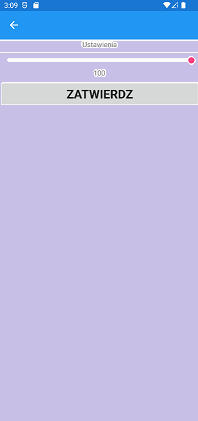
\includegraphics[width=8cm]{rys/ustawienia.png}
		\caption{Ustawienia}
		\label{rys:rysunek001}
	\end{center}
\end{figure}


\subsubsection{Tryb graficzny}
Pierwsza zagadka w trybie graficznym będzie wyglądała tak jak na rys 3.10.
Pomarańczowy kwdrat jest naszą postacią, którą poruszamy za pomocą strzałek umieszczonych na ekranie.
Każda strzałka odpowiada za ruch w inną stronę.
\\
\\
\\
\\
\\
\\
\\
\\
\\
\\
\\
\\
\\
\\
\\
\\
\\
	\begin{figure}[!htb]
	\begin{center}
		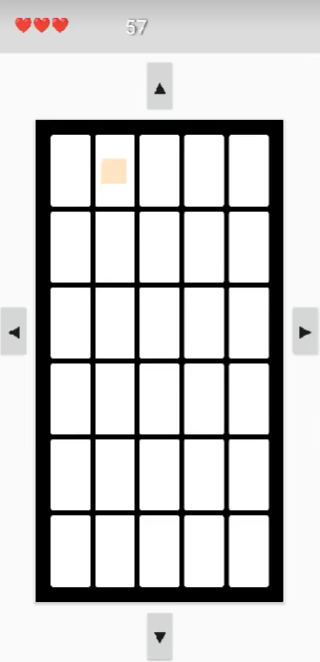
\includegraphics[width=8cm]{rys/gra7.png}
		\caption{Labirynt}
		\label{rys:rysunek001}
	\end{center}
\end{figure}
\\
Drugą zagadką będą "Literaki" (rys 3.11). Zagadka ta będzie polegała na ułożeniu odpowiedniego słowa. Za pomocą strzałek będziemy mogli zamieniać litery na odpowiednich polach. Przycisk z "ptaszkiem"~pozwoli nam sprawdzić ułożone słowo. 
\\
\\
\\
\\
	\begin{figure}[!htb]
	\begin{center}
		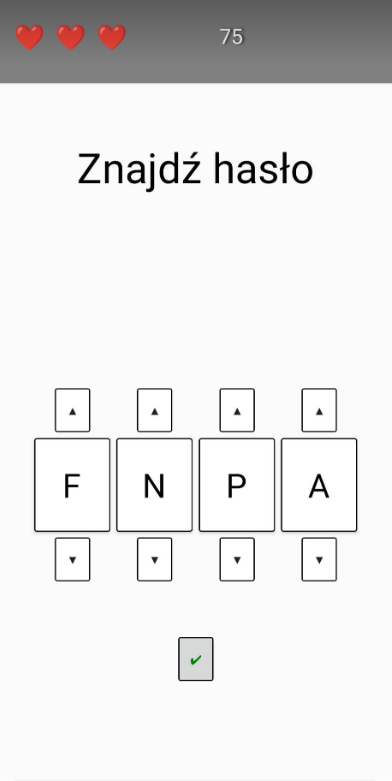
\includegraphics[width=8cm]{rys/gra88.png}
		\caption{Literaki}
		\label{rys:rysunek001}
	\end{center}
\end{figure}

\hspace{-0.60cm}Kolejna zagadka będzie polegała na wyborze odpowiedniego słowa, będziemy zamieniać litery za pomocą strzałek jak na rys 3.12. Jeżeli ułożymy odpowiednie słowo zatwierdzamy przyciskem oznaczonym "ptaszkiem". Za pomocą przycisku odtwórz możemy odtworzyć kod morsa z latarki od nowa. 
\\
\\
\\
\\
\\
\\
	\begin{figure}[!htb]
	\begin{center}
		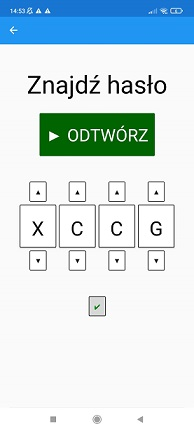
\includegraphics[width=8cm]{rys/gra8.png}
		\caption{Kod morsa}
		\label{rys:rysunek001}
	\end{center}
\end{figure}

\hspace{-0.60cm}Następna zagadka (rys 3.13) będzie polegała na wypatrywaniu jaki kolor został wyróżniony po czym kliknięcie w odpowiadający mu inny. Zagadka w zamyśle jest porosta ale testu pamięć i spostrzegawczość osoby grającej w trybie graficznym.
\\
\\
\\
\\
	\begin{figure}[!htb]
	\begin{center}
		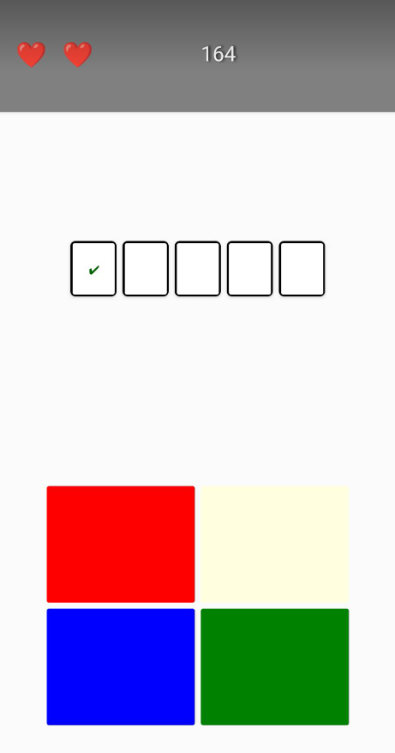
\includegraphics[width=8cm]{rys/gra99.png}
		\caption{Kolorki}
		\label{rys:rysunek001}
	\end{center}
\end{figure}

\hspace{-0.60cm}Ostatnia zagadka będzie najprostsza (rys 3.14). Będzie polegała na spostrzeżeniu koloru przycisku i przytrzymaniu go przez określony czas. 

	\begin{figure}[!htb]
	\begin{center}
		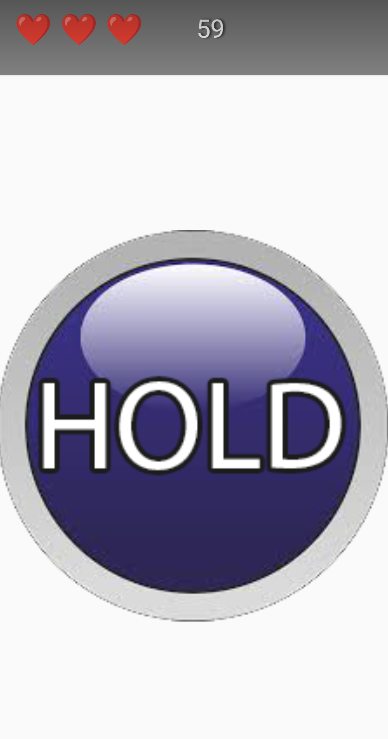
\includegraphics[width=8cm]{rys/gra666.png}
		\caption{Wielki Przycisk}
		\label{rys:rysunek001}
	\end{center}
\end{figure}
